% !TeX TS-program = xelatex
% !Mode TeXUTF-8
%# -- codingutf-8 --
% !TeX encoding = UTF-8
%%%%%%%%%%%%%%%%%%%%%%%%%%%%%%%%%%%%%%%%%%

\large\zihao{-4}
%---------------------------------------
\chapter{正定矩阵及其性质}\label{sec:2two}
%---------------------------------------
\section{预备知识}
\begin{definition}
设$A\in \mathbb{R}^{n\times n}$,若$A=A^T$,对任意的$0\neq x \in \mathbb{R}^{n\times 1}$,的、均有$x^{T}Ax>0$,则称$A$为实对称正定矩阵。
\end{definition}
\begin{lemma}

\end{lemma}
\section{正定矩阵的性质}

\LaTeX 文件的输入要涉及到一些 \LaTeX 命令，尤其是数学符号和公式的输入。这里通过实例来说明如何输入一些与数学有关的内容。建议学生在使用前阅读一遍。通过对比PDF文件中的效果和源文件对应的排版命令，初学者可以快速上手使用\LaTeX 。
\begin{definition}
设
\begin{equation}\label{eq:1}
    a_1,a_2,\cdots, a_n, \cdots
\end{equation}
是一个数列。称
$$\sum_{i=1}^n a_i$$
为数列~\eqref{eq:1} 的前$n$项和\index{前$n$项和}。
\end{definition}
\begin{lemma}[新定理]
若$p$是一个素数，且$p$不能够被$a\in \mathbb{N}$整除，则
$$a^{p-1}\equiv 1\pmod{p}.$$
\end{lemma}
\begin{proof}
引理的证明在此给出。
\end{proof}
\begin{theorem}[欧拉定理\index{欧拉定理}]\label{thm:euola}
若$\gcd(a,n) = 1$，则
$$a^{\phi(n)}\equiv 1\pmod{n}.$$
\end{theorem}
\begin{proof}
下面我们来证明这个定理。
\end{proof}
\begin{lemma}[费尔马小定理\index{费尔马小定理}]
若$p$是一个素数\index{素数}，且$p$不能够被$a\in \mathbb{N}$整除，则
$$a^{p-1}\equiv 1\pmod{p}.$$
\end{lemma}
\begin{proof}
引理的证明在此给出。
\end{proof}
\begin{corollary} 由组合数的定义立得
$$\binom{n}{k}=\binom{n}{n-k}.$$
\end{corollary}
\begin{property}
设线性变换$\mathscr{A}$在基$\bm{\alpha}_1,\bm{\alpha}_2,\cdots,\bm{\alpha}_n$下矩阵为
\[
\begin{pmatrix}
 a_{11} & a_{12} & \cdots & a_{1n} \\
 a_{21} & a_{22} & \cdots & a_{2n} \\
 \vdots & \vdots &        & \vdots \\
 a_{n1} & a_{n2} & \cdots & a_{nn}
\end{pmatrix},
\]
向量$\bm{\alpha}$在基$\bm{\alpha}_1,\bm{\alpha}_2,\cdots,\bm{\alpha}_n$下的坐标为$ (x_1,x_2,\cdots,x_n)$. 则$\mathscr{A}\bm{\alpha}$在基$\bm{\alpha}_1,\bm{\alpha}_2,\cdots,\bm{\alpha}_n$下的坐标$(y_1,y_2,\cdots,y_n)$可以按公式
\[
\begin{pmatrix}
y_1 \\
y_2 \\
\vdots \\
y_n
\end{pmatrix} = 
\begin{pmatrix}
a_{11} & a_{12} & \cdots & a_{1n} \\
a_{21} & a_{22} & \cdots & a_{2n} \\
\vdots & \vdots &        & \vdots \\
a_{n1} & a_{n2} & \cdots & a_{nn}
\end{pmatrix} 
\begin{pmatrix}
x_1 \\
x_2 \\
\vdots \\
x_n
\end{pmatrix}
\]
计算.
\end{property}
%\begin{example}[2011\ 江苏卷]在平面直角坐标系$xOy$中，$M$,$N$分别是椭圆$C$：
%$\frac{x^{2}}{4^{2}}+\frac{y^{2}}{2^{2}}=1$的顶点，
%过坐标原点的直线交椭圆于$P$,$A$两点，其中点$P$在第一象限.过$P$ 作$x$轴的垂线，
%垂足为$C$.连接$AC$，并延长交椭圆与点$B$.设直线$PA$的斜率为$k$.\\
%\parbox{10cm}{
%\begin{enumerate}
%  \item 若直线$PA$平分线段$MN$，求$k$的值；
%  \item 当$k=2$时，求点$P$到直线$AB$的距离$d$；
%  \item 对任意的$k>0$，求证：$PA\perp PB$.
%\end{enumerate}}
%\parbox{3cm}{
%\begin{center}
%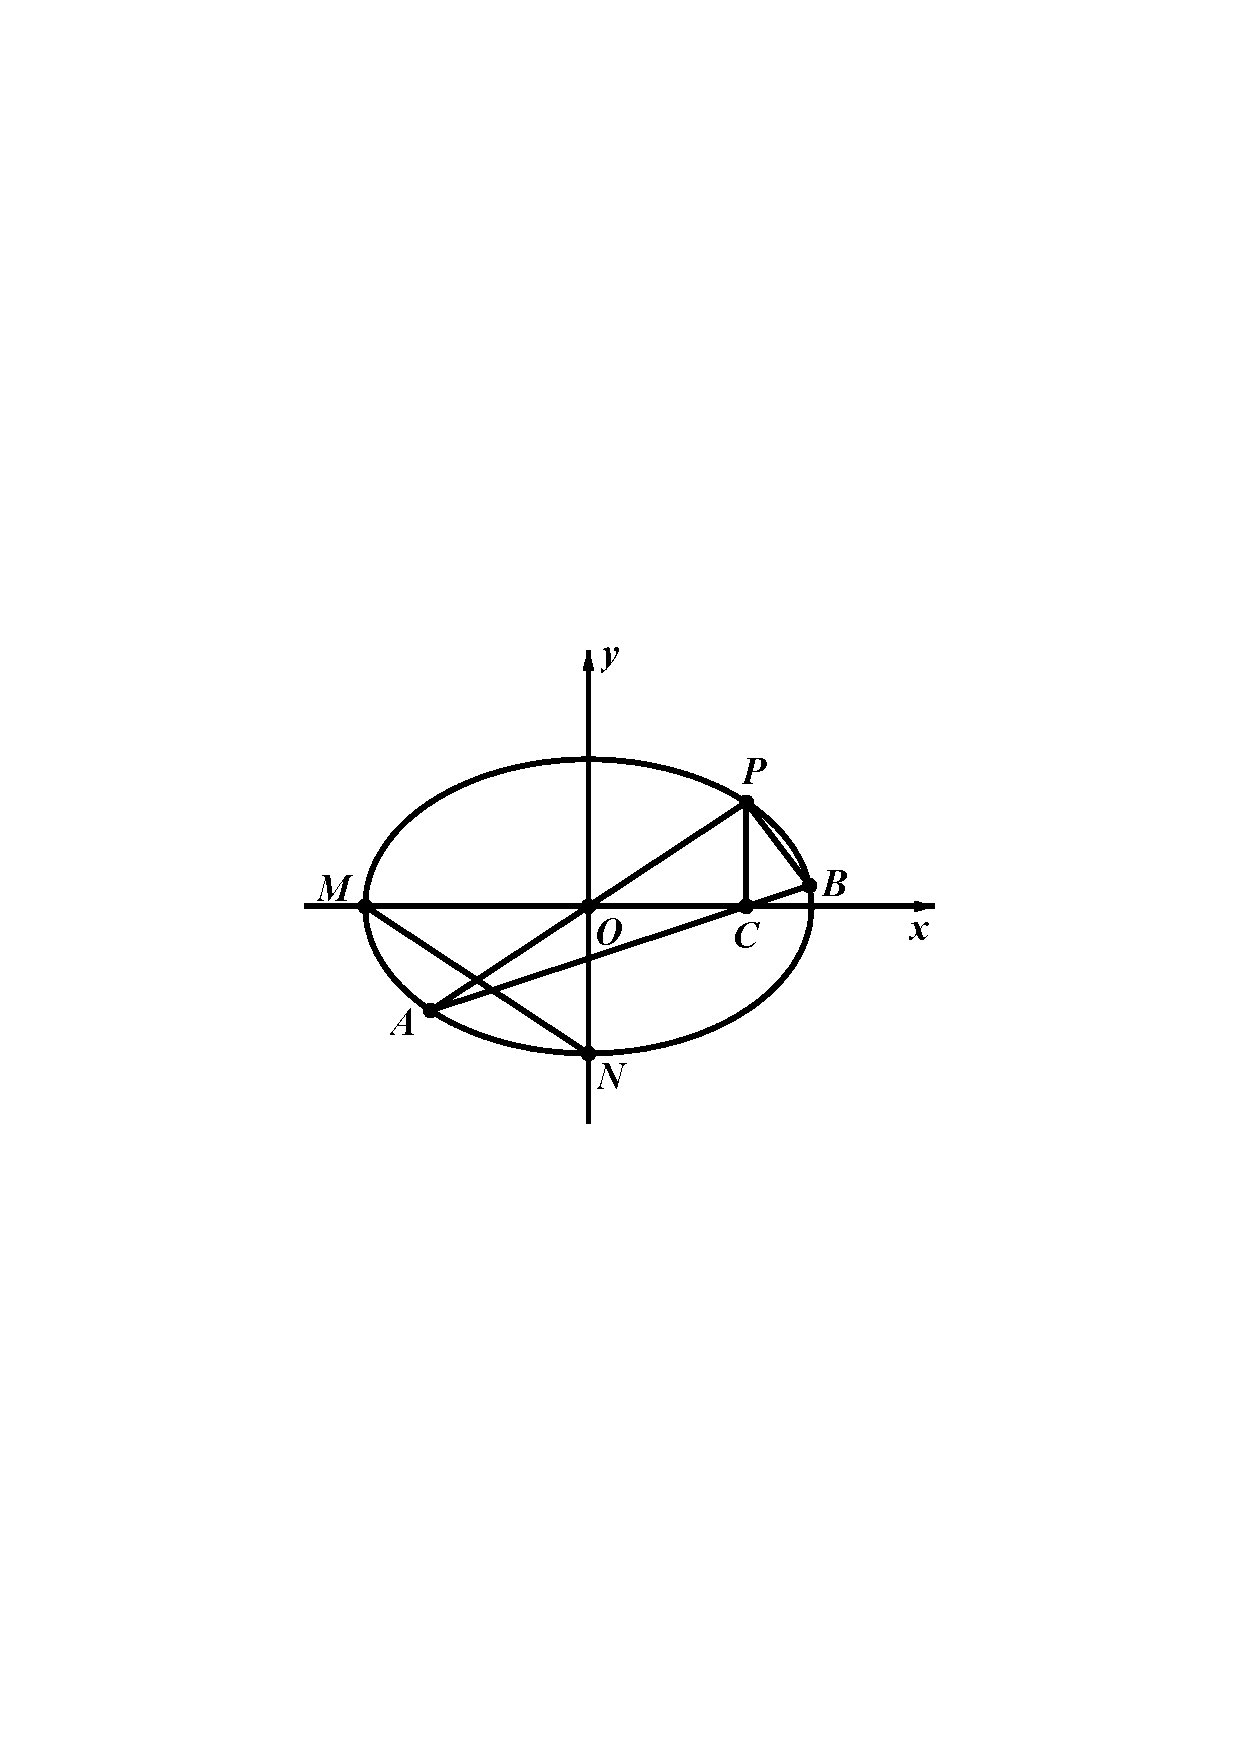
\includegraphics[height=3cm,angle=0]{figs/wangyang_2}\\
%%\caption{椭圆}\label{fig:1}
%\end{center}}
%\end{example}

\begin{example}[2010，重庆卷]
例题的内容$\langle ID,\mu,\gamma\rangle$，$\langle ID,\mu,\gamma\rangle$。
\end{example}
\begin{solution}
解答的内容。
\end{solution}
\begin{exercise}
练习题的内容。
\end{exercise}
\begin{note}
设
\[
D =
\begin{vmatrix}
  5 & 1 & -1 \\
  -7 & 1 & 15 \\
  8 & 1 & -21 \\
\end{vmatrix}
\]
则$D$的第$3$列元的代数余子式的和是$0$。
\end{note}
\begin{proposition}
计算$\displaystyle\int_0^1 \dfrac{x}{\sqrt{1-x^2}} {\rm d}x$。
\end{proposition}
\begin{solution}
因为
$$\int_0^u\frac{x}{\sqrt{1-x^2}} {\rm d}x = -\int_0^u\frac{ {\rm d}(1-x^2)}{2\sqrt{1-x^2}} = \left.-\sqrt{1-x^2}\right|_0^u = 1-\sqrt{1-u^2},$$
所以$\displaystyle\int_0^u\frac{x}{\sqrt{1-x^2}} {\rm d}x = \lim_{u\rightarrow 1^{-}}\int_0^u\frac{x}{\sqrt{1-x^2}} {\rm d}x = 1$。
\end{solution}
\section{矩阵的排版}
分块矩阵的排版示例如下：
\[
\left[
\begin{array}{cc:cc}
a_{11} & a_{12} & b_{11} & b_{12}\\
a_{21} & a_{22} & b_{21} & b_{22}\\
\hdashline
c_{11} & c_{12} & d_{11} & d_{12}\\
c_{11} & c_{12} & d_{11} & d_{12}\\
\end{array}
\right]
\]
\[\mathbf{A} =
\bordermatrix{
      & n_1             & n_2             & \cdots & n_l \cr
  s_1 & \mathbf{A}_{11} & \mathbf{A}_{12} & \cdots & \mathbf{A}_{1l}\cr
  s_2 & \mathbf{A}_{21} & \mathbf{A}_{22} & \cdots & \mathbf{A}_{2l}\cr
  \vdots & \vdots       &        \vdots   &        & \vdots \cr
  s_t & \mathbf{A}_{t1} & \mathbf{A}_{t2} & \cdots & \mathbf{A}_{tl}\cr
}
\]
%A = \begin{pmat}[{..|..}]
%a_{11} & a_{12} & a_{13} & a_{14} & a_{15}\cr
%a_{21} & a_{22} & a_{23} & a_{24} & a_{25}\cr\-
%a_{31} & a_{32} & a_{33} & a_{34} & a_{35}\cr
%\end{pmat},
%$$
\section{算法的排版}
用~\LaTeX{} 可以排出版面非常漂亮的算法\index{算法的排版}。根据所用宏包\index{宏包}的不同，所用的命令也有所不同。下面是用宏包~{\tt algorithm} 和~{\tt algorithmic} 进行算法排版的一个例子。所排的算法是著名的\index{欧几里得算法}欧几里得算法\citeu{stinson}。

%%%%%%%%%%%%%%%%%%%%%%%%%%%%%%%%%%%%%%%%%%%%%%%
\begin{algorithm}
\caption{Euclidean algorithm$(a,b)$}
\label{alg:euclid}
\algsetup{indent=2em}
\begin{algorithmic}[1]
\REQUIRE 整数$a,b\ne 0$
\ENSURE  商序列$q_1,q_2,\cdots,q_m$和$\gcd(a,b)$
\STATE $r_0 \leftarrow a$
\STATE $r_1 \leftarrow b$
\STATE $m\leftarrow 1$
\WHILE{$r_m\ne 0$}
\STATE $q_m\leftarrow\lfloor\frac{r_{m-1}}{r_m}\rfloor$
\STATE $r_m\leftarrow r_{m-1}-q_mr_m$
\STATE $m\leftarrow m+1$
\ENDWHILE
\STATE $m\leftarrow m-1$
\RETURN {$(q_1,q_2,\cdots, q_m;r_m)$}
\STATE {\bf{comment：}$r_m = \gcd(a,b)$ }
\end{algorithmic}
\end{algorithm}
算法~\ref{alg:euclid_no} 是另一个标号\index{算法标号}的。
\begin{algorithm}
\caption{Euclidean algorithm$(a,b)$}
\label{alg:euclid_no}
\algsetup{indent=2em}
\begin{algorithmic}[2]
\REQUIRE 整数$a,b\ne 0$
\ENSURE  商序列$q_1,q_2,\cdots,q_m$和$\gcd(a,b)$
\STATE $r_0 \leftarrow a$
\STATE $r_1 \leftarrow b$
\STATE $m\leftarrow 1$
\WHILE{$r_m\ne 0$}
\STATE $q_m\leftarrow\lfloor\frac{r_{m-1}}{r_m}\rfloor$
\STATE $r_m\leftarrow r_{m-1}-q_mr_m$
\STATE $m\leftarrow m+1$
\ENDWHILE
\STATE $m\leftarrow m-1$
\RETURN {$(q_1,q_2,\cdots, q_m;r_m)$}
%\STATE {\bf{comment：}$r_m = \gcd(a,b)$ }
\end{algorithmic}
\end{algorithm}

%\setcounter{algorithm}{4}
下面的算法~\ref{alg:rgg} 是一个生成$q$进制$n$元反射Gray码\index{反射Gray码}的算法。
\begin{algorithm}
\caption{\sc Reflected Gray Code Generation$(q, n)$}
\label{alg:genGraycode}
\algsetup{indent=2em}
\begin{algorithmic}
%%\TitleOfAlgo{Euclidean algorithm$(a,b)$}
\label{alg:rgg}
\REQUIRE{整数$q>0,n > 0$}
\ENSURE {$q^n\times n$矩阵$G$}
\STATE $g_{n-1}g_{n-2}\cdots g_{0}\longleftarrow 00\cdots 0$
\WHILE{$(2\mid q$ \AND $g_{n-1},g_{n-2},\cdots ,g_{0} \neq q-1,\bm{0}_{n-1})$ \OR $(2\nmid q$ \AND $g_{n-1},\cdots ,g_{n} \neq \bm{(q-1)}_{n}$}
    \STATE $i\leftarrow 0$
    \STATE $\sigma \leftarrow (g_{n-1}+g_{n-2}+\cdots +g_{i+1})\bmod 2$
    \IF{$\sigma=0$ \AND $g_{i}\neq q-1$}
        \STATE $g_{i} \leftarrow g_{i}+1$
    \ELSIF{$\sigma =1$ \AND $g_{i}\neq 0$}
        \STATE $g_{i}\leftarrow g_{i}-1$
    \ENDIF
    \STATE $i \leftarrow i+1$
    \IF{$i = q-1$}
        \STATE $g_{i} \leftarrow g_{i}+1$
    \ENDIF
\ENDWHILE
\end{algorithmic}
\end{algorithm}
%再来一个不标号不连线的：
%\LinesNotNumbered
%\SetAlgoNoLine
%
%\begin{procedure}[H]
%\caption{$f$()\hspace{-.15cm}$(x,a,b)$}
%\label{proc:f}
%\KwIn{$x,a,b$}
%\uIf{$x\in S_1$}{
%    $f\leftarrow (\beta x,a,(b+1)\bmod n)$
%    }
%\uElseIf{$x\in S_2$}{
%    $f\leftarrow (x^2,2a\bmod n,2b\bmod n)$
%    }
%\Else{
%    $f\leftarrow (\alpha x,(a+1)\bmod n,b)$
%    }
%\Return{$(f)$}
%\end{procedure}
\begin{algorithm}
%\COMMENT{external}% {\bf  External: }}
%\begin{algorithmic}
\caption{{\sc Collision-To-Second-Preimage}\,$(h)$}
\label{algo:c2sec}
\begin{algorithmic}
%\REQUIRE{Hash 函数$h$}
\STATE \bf{External: }{\sc Oracle-2nd-Preimage}
\STATE Choose $x\in_R\mathcal{X}$
\IF{{\sc Oracle-2nd-Preimage}\,$(h,x) = x'$}
    \RETURN $(x,x')$
\ELSE{\RETURN{{\rm(``failure")}}}
\ENDIF
\end{algorithmic}
\end{algorithm}
